\section{ShowCase}


Um das  Projekt zu starten, muss auf den Ordner 'Drowsiness detection' zugegriffen werden und die Py Datei, 'drowsiness detection.py' ausgeführt werden.

Dies geschieht alles in CMD.

\begin{lstlisting}
1. cd 'Drowsiness detection'

2. Python 'drowsiness detection.py'

\end{lstlisting}


Folgend wird in der Py Datei 'dorwsiness detection auf die Unten dargestellten Dateien zugegriffen.


\begin{figure}[htbp]
  \centering
     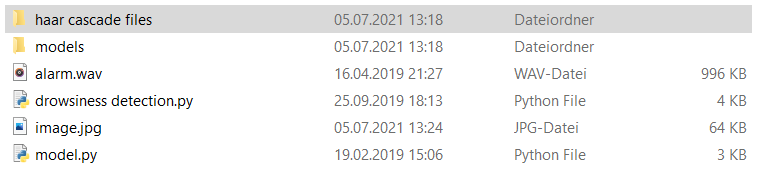
\includegraphics[width=0.48\textwidth]{Dateien.png}
     \caption{Dateien}
\end{figure}

Im 'haar cascade files', befinden sich die xml Dateien, 
die benötigt werden um die Gesichter und Augen zu erkennen.


Der 'models' Ordner enthält das model fiel 'cnn.Cat2.h5', 
für das mehrdimensionale Array im 'Convolutional neural network'. 

Zur Erkennung der Details im Bild.


Zudem beinhaltet der Ordern die 'alarm.wav' Datei,
um das Warnsignal abzuspielen, wenn der kritische Wert erreicht ist.


'Drowsiness detection' ist die Hauptdatei zum starten des Programmablaufes.


In dem Python Code, werden die einzelnen Dateien aufgerufen und ausgeführt.
\newpage
\begin{lstlisting}
model = load_model('models/cnncat2.h5')

sound = mixer.Sound('alarm.wav')


face = cv2.CascadeClassifier

('haar cascade files
\haarcascade_frontalface_alt.xml')

leye = cv2.CascadeClassifier

('haar cascade files
\haarcascade_lefteye_2splits.xml')

reye = cv2.CascadeClassifier

('haar cascade files
\haarcascade_righteye_2splits.xml')

\end{lstlisting} 

Um das das vollständige Programm zu starten.\cite{b1}

\subsection{Beispiel}

\begin{figure}[htbp]
  \centering
     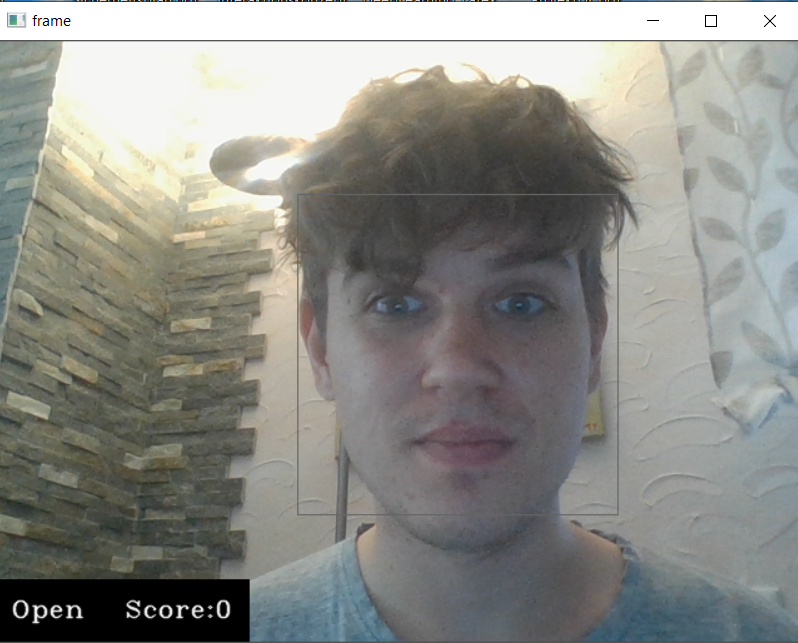
\includegraphics[width=0.35\textwidth]{Open.png}
     \caption{Open}
\end{figure}

Auf dem Bild ist zu sehen, dass das Gesicht der Person erkannt wird.

Es wird festgestellt, dass die Augen geöffnet(open) sind.

Der Score befindet sich deshalb bei '0' und sendet kein Geräusch aus.

\begin{figure}[htbp]
  \centering
     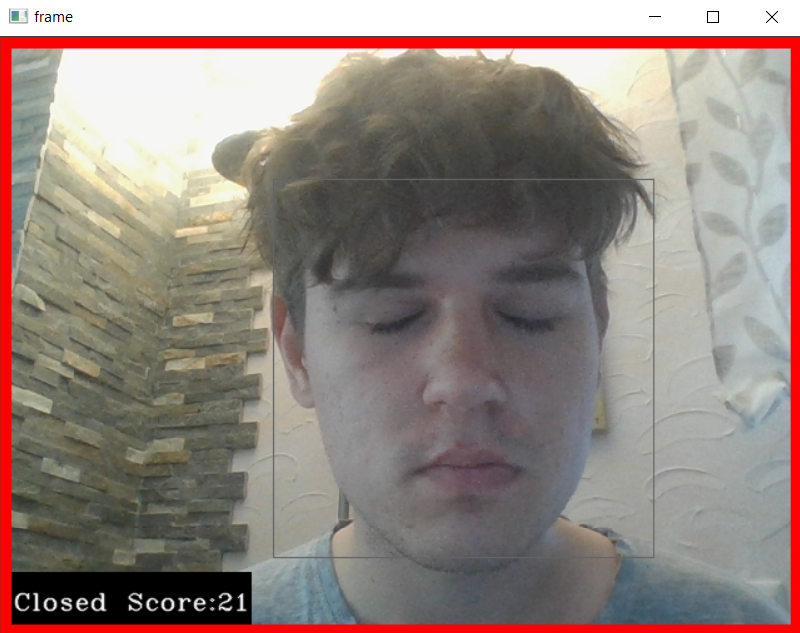
\includegraphics[width=0.35\textwidth]{Closed.png}
     \caption{Closed}
\end{figure}

Im nächsten Bild ist zu erkennen, dass die Augen der Person geschlossen (closed) sind.

So wird der Score hochgezählt und der Rand zeigt ein Warnzeichen an mit einer roten Umrandung.

Zum Schluss wird ab einem Score von '15' ein Warnsignal abgespielt.
\newline
\newline